\documentclass[11pt,letterpaper,twoside]{report}

%%%%%%%%%%%%%%%%%%%%%%%%%%%%%%%%%%%%%%%%%%%%%%%%%%
%% DEBUG / LAYOUT TOOLS
%%%%%%%%%%%%%%%%%%%%%%%%%%%%%%%%%%%%%%%%%%%%%%%%%%

% Toggle layout grid for debugging margins
%\def\showGrid{1}
\def\showGrid{0}
\if\showGrid1
    \usepackage[grid,gridunit=in,subgridcolor=blue!20]{eso-pic}
    \usepackage[grid,gridunit=in,subgridcolor=blue!20]{showframe}
\fi

%%%%%%%%%%%%%%%%%%%%%%%%%%%%%%%%%%%%%%%%%%%%%%%%%%
%% PAGE LAYOUT & SPACING
%%%%%%%%%%%%%%%%%%%%%%%%%%%%%%%%%%%%%%%%%%%%%%%%%%

\usepackage{geometry}
\usepackage{setspace}
\usepackage{titlesec}
\usepackage[subfigure]{tocloft}

% Chapter formatting in TOC
\renewcommand{\cftchappresnum}{CHAPTER }
\renewcommand{\cftchapaftersnum}{: }
\setlength{\cftchapnumwidth}{6.5em}

\setlength{\footskip}{0.5in}

%%%%%%%%%%%%%%%%%%%%%%%%%%%%%%%%%%%%%%%%%%%%%%%%%%
%% LISTS & TEXT FORMATTING
%%%%%%%%%%%%%%%%%%%%%%%%%%%%%%%%%%%%%%%%%%%%%%%%%%

\usepackage{enumerate}
\usepackage{enumitem}
\usepackage[normalem]{ulem}   % underline support
\usepackage{etoolbox}         % patching commands
\usepackage{paralist}         % inline lists (inparaenum)

% Allow line breaks in underlined text
\makeatletter
\patchcmd{\UL@word}{\space}{\space\allowbreak}{}{}
\makeatother

%%%%%%%%%%%%%%%%%%%%%%%%%%%%%%%%%%%%%%%%%%%%%%%%%%
%% FOOTNOTES
%%%%%%%%%%%%%%%%%%%%%%%%%%%%%%%%%%%%%%%%%%%%%%%%%%

\usepackage[hang,flushmargin]{footmisc}

%%%%%%%%%%%%%%%%%%%%%%%%%%%%%%%%%%%%%%%%%%%%%%%%%%
%% GLOSSARY / ACRONYMS
%%%%%%%%%%%%%%%%%%%%%%%%%%%%%%%%%%%%%%%%%%%%%%%%%%

\usepackage[acronym,nonumberlist]{glossaries}
% common/acronyms.tex

\newacronym{UNC}{UNC}{University of North Carolina}
\newacronym{HMSC}{HMSC}{Human Movement Science Curriculum}
\newacronym{GDTBATH}{GDTBATH}{Great Day to Be A Tarheel}
% \makeglossaries  % Uncomment if building glossary list

%%%%%%%%%%%%%%%%%%%%%%%%%%%%%%%%%%%%%%%%%%%%%%%%%%
%% BIBLIOGRAPHY
%%%%%%%%%%%%%%%%%%%%%%%%%%%%%%%%%%%%%%%%%%%%%%%%%%

\usepackage[citestyle=ama, bibstyle=ama]{biblatex}
\addbibresource{diss.bib}

% Prevent overfull lines in bibliography
\AtBeginBibliography{%
  \sloppy
  \emergencystretch=2em
}

%%%%%%%%%%%%%%%%%%%%%%%%%%%%%%%%%%%%%%%%%%%%%%%%%%
%% FIGURES & GRAPHICS
%%%%%%%%%%%%%%%%%%%%%%%%%%%%%%%%%%%%%%%%%%%%%%%%%%

\usepackage{graphicx}
\usepackage{float}
\usepackage{subfigure}
\usepackage{multicol}

%%%%%%%%%%%%%%%%%%%%%%%%%%%%%%%%%%%%%%%%%%%%%%%%%%
%% TABLES
%%%%%%%%%%%%%%%%%%%%%%%%%%%%%%%%%%%%%%%%%%%%%%%%%%

\usepackage{tabularx}

% Column alignment helpers
\newcommand{\tr}{\raggedright\arraybackslash}
\newcommand{\tc}{\centering\arraybackslash}
\newcommand{\tl}{\raggedleft\arraybackslash}

\usepackage{caption}
\captionsetup{
  labelfont=bf,
  labelsep=period
}

% Supplementary figures
\DeclareCaptionType{supfigure}[Supplementary Figure][List of Supplementary Figures]

%%%%%%%%%%%%%%%%%%%%%%%%%%%%%%%%%%%%%%%%%%%%%%%%%%
%% ALGORITHMS
%%%%%%%%%%%%%%%%%%%%%%%%%%%%%%%%%%%%%%%%%%%%%%%%%%

\usepackage[boxed,longend]{algorithm2e}

%%%%%%%%%%%%%%%%%%%%%%%%%%%%%%%%%%%%%%%%%%%%%%%%%%
%% MATH
%%%%%%%%%%%%%%%%%%%%%%%%%%%%%%%%%%%%%%%%%%%%%%%%%%

\usepackage{amsmath}
\usepackage{amssymb}
\usepackage{mathtools}

%%%%%%%%%%%%%%%%%%%%%%%%%%%%%%%%%%%%%%%%%%%%%%%%%%
%% TYPOGRAPHY
%%%%%%%%%%%%%%%%%%%%%%%%%%%%%%%%%%%%%%%%%%%%%%%%%%

\usepackage{times}
\usepackage{microtype}
\usepackage{textcomp}
\usepackage{rotating}
\usepackage{adjustbox}

%%%%%%%%%%%%%%%%%%%%%%%%%%%%%%%%%%%%%%%%%%%%%%%%%%
%% UTILITIES / MACROS
%%%%%%%%%%%%%%%%%%%%%%%%%%%%%%%%%%%%%%%%%%%%%%%%%%

\usepackage{xspace}
\usepackage{color}
\usepackage{ntheorem}
\usepackage{siunitx}

%%%%%%%%%%%%%%%%%%%%%%%%%%%%%%%%%%%%%%%%%%%%%%%%%%
%% DIAGRAMS (TikZ)
%%%%%%%%%%%%%%%%%%%%%%%%%%%%%%%%%%%%%%%%%%%%%%%%%%

\usepackage{tikz}
\usetikzlibrary{calc, positioning, arrows.meta, trees}

%%%%%%%%%%%%%%%%%%%%%%%%%%%%%%%%%%%%%%%%%%%%%%%%%%
%% HYPERLINKS & PDF FEATURES
%%%%%%%%%%%%%%%%%%%%%%%%%%%%%%%%%%%%%%%%%%%%%%%%%%

\usepackage[hidelinks]{hyperref}
\usepackage{pdfcomment}

% Glossary tooltip behavior:
% - First use = full term
% - Subsequent use = abbreviation + hover definition
\let\oldgls\gls
\renewcommand{\gls}[1]{%
  \ifglsused{#1}
    {\pdftooltip{\oldgls{#1}}{\glsentrylong{#1}}}
    {\oldgls{#1}}%
}

%%%%%%%%%%%%%%%%%%%%%%%%%%%%%%%%%%%%%%%%%%%%%%%%%%
%% CUSTOM LAYOUT + MACROS
%%%%%%%%%%%%%%%%%%%%%%%%%%%%%%%%%%%%%%%%%%%%%%%%%%

\input{common/layout}
\input{common/macros}

%%%%%%%%%%%%%%%%%%%%%%%%%%%%%%%%%%%%%%%%%%%%%%%%%%
%% DOCUMENT START
%%%%%%%%%%%%%%%%%%%%%%%%%%%%%%%%%%%%%%%%%%%%%%%%%%

\begin{document}

% Front matter (title, TOC, etc.)
\input{frontmatter/pages}

% Chapters
\chapter{Introduction}\label{chap:introduction}

% This creates a chapter and assigns a label for cross-referencing:
% you can later refer to it using \autoref{chap:introduction}

\section{Purpose of This Template}

This chapter demonstrates the basic structure of a dissertation written in \LaTeX{}. It shows how to organize text into chapters and sections, how to include citations, and how to use glossary terms consistently throughout a document.

Sections (created using \texttt{\textbackslash section\{\}}) divide content into logical units. Each section should represent a coherent idea or topic.

\section{Working with Citations}

Citations are inserted using commands such as \texttt{\textbackslash supercite\{\}}. These commands pull references directly from your bibliography file (e.g., \texttt{.bib} file) and format them automatically.

For example, you can cite prior work like this.\supercite{example_reference_1}

Using citation commands ensures consistency in formatting and allows you to easily update or change citation styles without editing text manually.

\section{Conceptual Writing Example}

In many research domains, complex systems are characterized by interactions across multiple scales and levels of organization. Writing in an introduction should clearly motivate the problem, define key concepts, and situate the work within existing literature.\supercite{example_reference_2}

This section demonstrates how narrative text, citations, and structure work together to form a cohesive argument.

\section{Using Glossary Terms and Acronyms}

Glossary terms are defined in a separate file (e.g., \texttt{common/acronyms.tex}) and referenced using the \texttt{\textbackslash gls\{\}} command.

For example, \gls{UNC} refers to the Universirt of north carolina at chapel hill. But I could enter type "gls" again and now it is abbreviated \gls{UNC}.

It also works with \gls{GDTBATH}, which is especially great when we beat DOOK in basketball. You'll hear everyone say \gls{GDTBATH}.

One final example for \gls{HMSC}, our doctoral program. We like to say it the \gls{HMSC} program is interdisciplinary, and is housedin the \gls{UNC} school of medicine.

On first use, the full term is typically displayed (e.g., “electroencephalography (EEG)”), and on subsequent uses, only the abbreviation appears. In adobe acrobat PDF viewers, hovering over the term will display its definition.

This approach ensures consistent terminology throughout the document and is especially useful in fields with many abbreviations.

\section{General Writing Structure}

Structuring your writing in this way improves clarity and helps guide the reader through your argument.

\section{Summary}

This chapter demonstrated the foundational elements of writing in \LaTeX{}, including: \begin{inparaenum}[(i)]
    \item Chapter and section organization
    \item Citation usage with \texttt{\textbackslash supercite}
    \item Glossary term integration with \texttt{\textbackslash gls}
    \item General principles for structuring academic writing
\end{inparaenum}

These components form the basis for building more complex chapters in a dissertation.
\chapter{Review of the Literature}\label{chap:literature_review}

% Creates a chapter and allows referencing with \autoref{chap:literature_review}

\section{Example Section}

Lorem ipsum dolor sit amet, consectetur adipiscing elit.\supercite{example_reference_1}

% \supercite{} inserts a citation from your .bib file

The major components of this framework are summarized in \textbf{\autoref{tab:example_table}}.

% \autoref{} automatically formats the reference as "Table X"
% Always reference tables/figures in text before they appear

\begin{table}[H]
\setstretch{1.0} % Controls vertical spacing within the table
\centering % Centers the table on the page

\caption{Example Table Title for Demonstration Purposes. This caption appears in the List of Tables}
% Caption appears above the table (standard for dissertations)

\label{tab:example_table}
% Label MUST come after caption for correct cross-referencing

\begin{tabular}{p{3.1cm} p{3.5cm} p{6.55cm}}
% Defines column layout:
% p{} creates fixed-width columns with automatic text wrapping
% This is preferred over l/c/r for long text in dissertations

\hline
\textbf{Category} & \textbf{Components} & \textbf{Description} \\
\hline

Example Row 1 
& Example Elements 
& Lorem ipsum dolor sit amet, consectetur adipiscing elit.\supercite{example_reference_1} 
\\

Example Row 2 
& Example Elements 
& Sed do eiusmod tempor incididunt ut labore et dolore magna aliqua.\supercite{example_reference_2} 
\\

Example Row 3 
& Example Elements 
& Ut enim ad minim veniam, quis nostrud exercitation ullamco laboris.\supercite{example_reference_3} 
\\

\hline
\hline

\multicolumn{3}{p{.95\linewidth}}{
\textit{Note.} This row spans all columns using \texttt{\textbackslash multicolumn}. 
Use this section for abbreviations, clarifications, or additional notes about the table.
}
\\

\hline
\end{tabular}
\end{table}

% Key table concepts:
% - Columns are separated by &
% - Rows end with \\
% - \hline creates horizontal rules
% - \multicolumn merges columns across the table width
% - p{} columns prevent text overflow and improve readability

Lorem ipsum dolor sit amet, consectetur adipiscing elit.

\section{Another Section}

An example glossary term is \gls{HMSC}.

% \gls{} pulls from the glossary file (e.g., common/acronyms.tex)
% First use = full term, subsequent uses = abbreviation

Example inline math: $p < 0.05$

% Inline math is used within a sentence

Example display math:

\[
y = mx + b
\]

% Display math is centered and used for emphasis or equations

\section{Summary}

Lorem ipsum dolor sit amet, consectetur adipiscing elit.
\chapter{Methods}\label{chap:methods}

% This creates a chapter and assigns a label so you can reference it elsewhere using \autoref{chap:methods}

This chapter outlines the general procedures used in this study. In a typical dissertation, the Methods chapter should provide enough detail for the study to be replicated, including participants, data acquisition, and analytic procedures.

\section{Study Overview}

% Sections break up your chapter logically

Lorem ipsum dolor sit amet, consectetur adipiscing elit.\supercite{example_reference_1}

% \supercite{} pulls from your .bib file and formats the citation automatically

As illustrated in \textbf{\autoref{fig:example_figure}}, the overall study workflow consists of multiple stages.

% \autoref{} automatically inserts the correct label (e.g., "Figure 1")
% Always reference figures/tables in text before they appear

\begin{figure}[htbp]
    \centering
    % Centers the image

    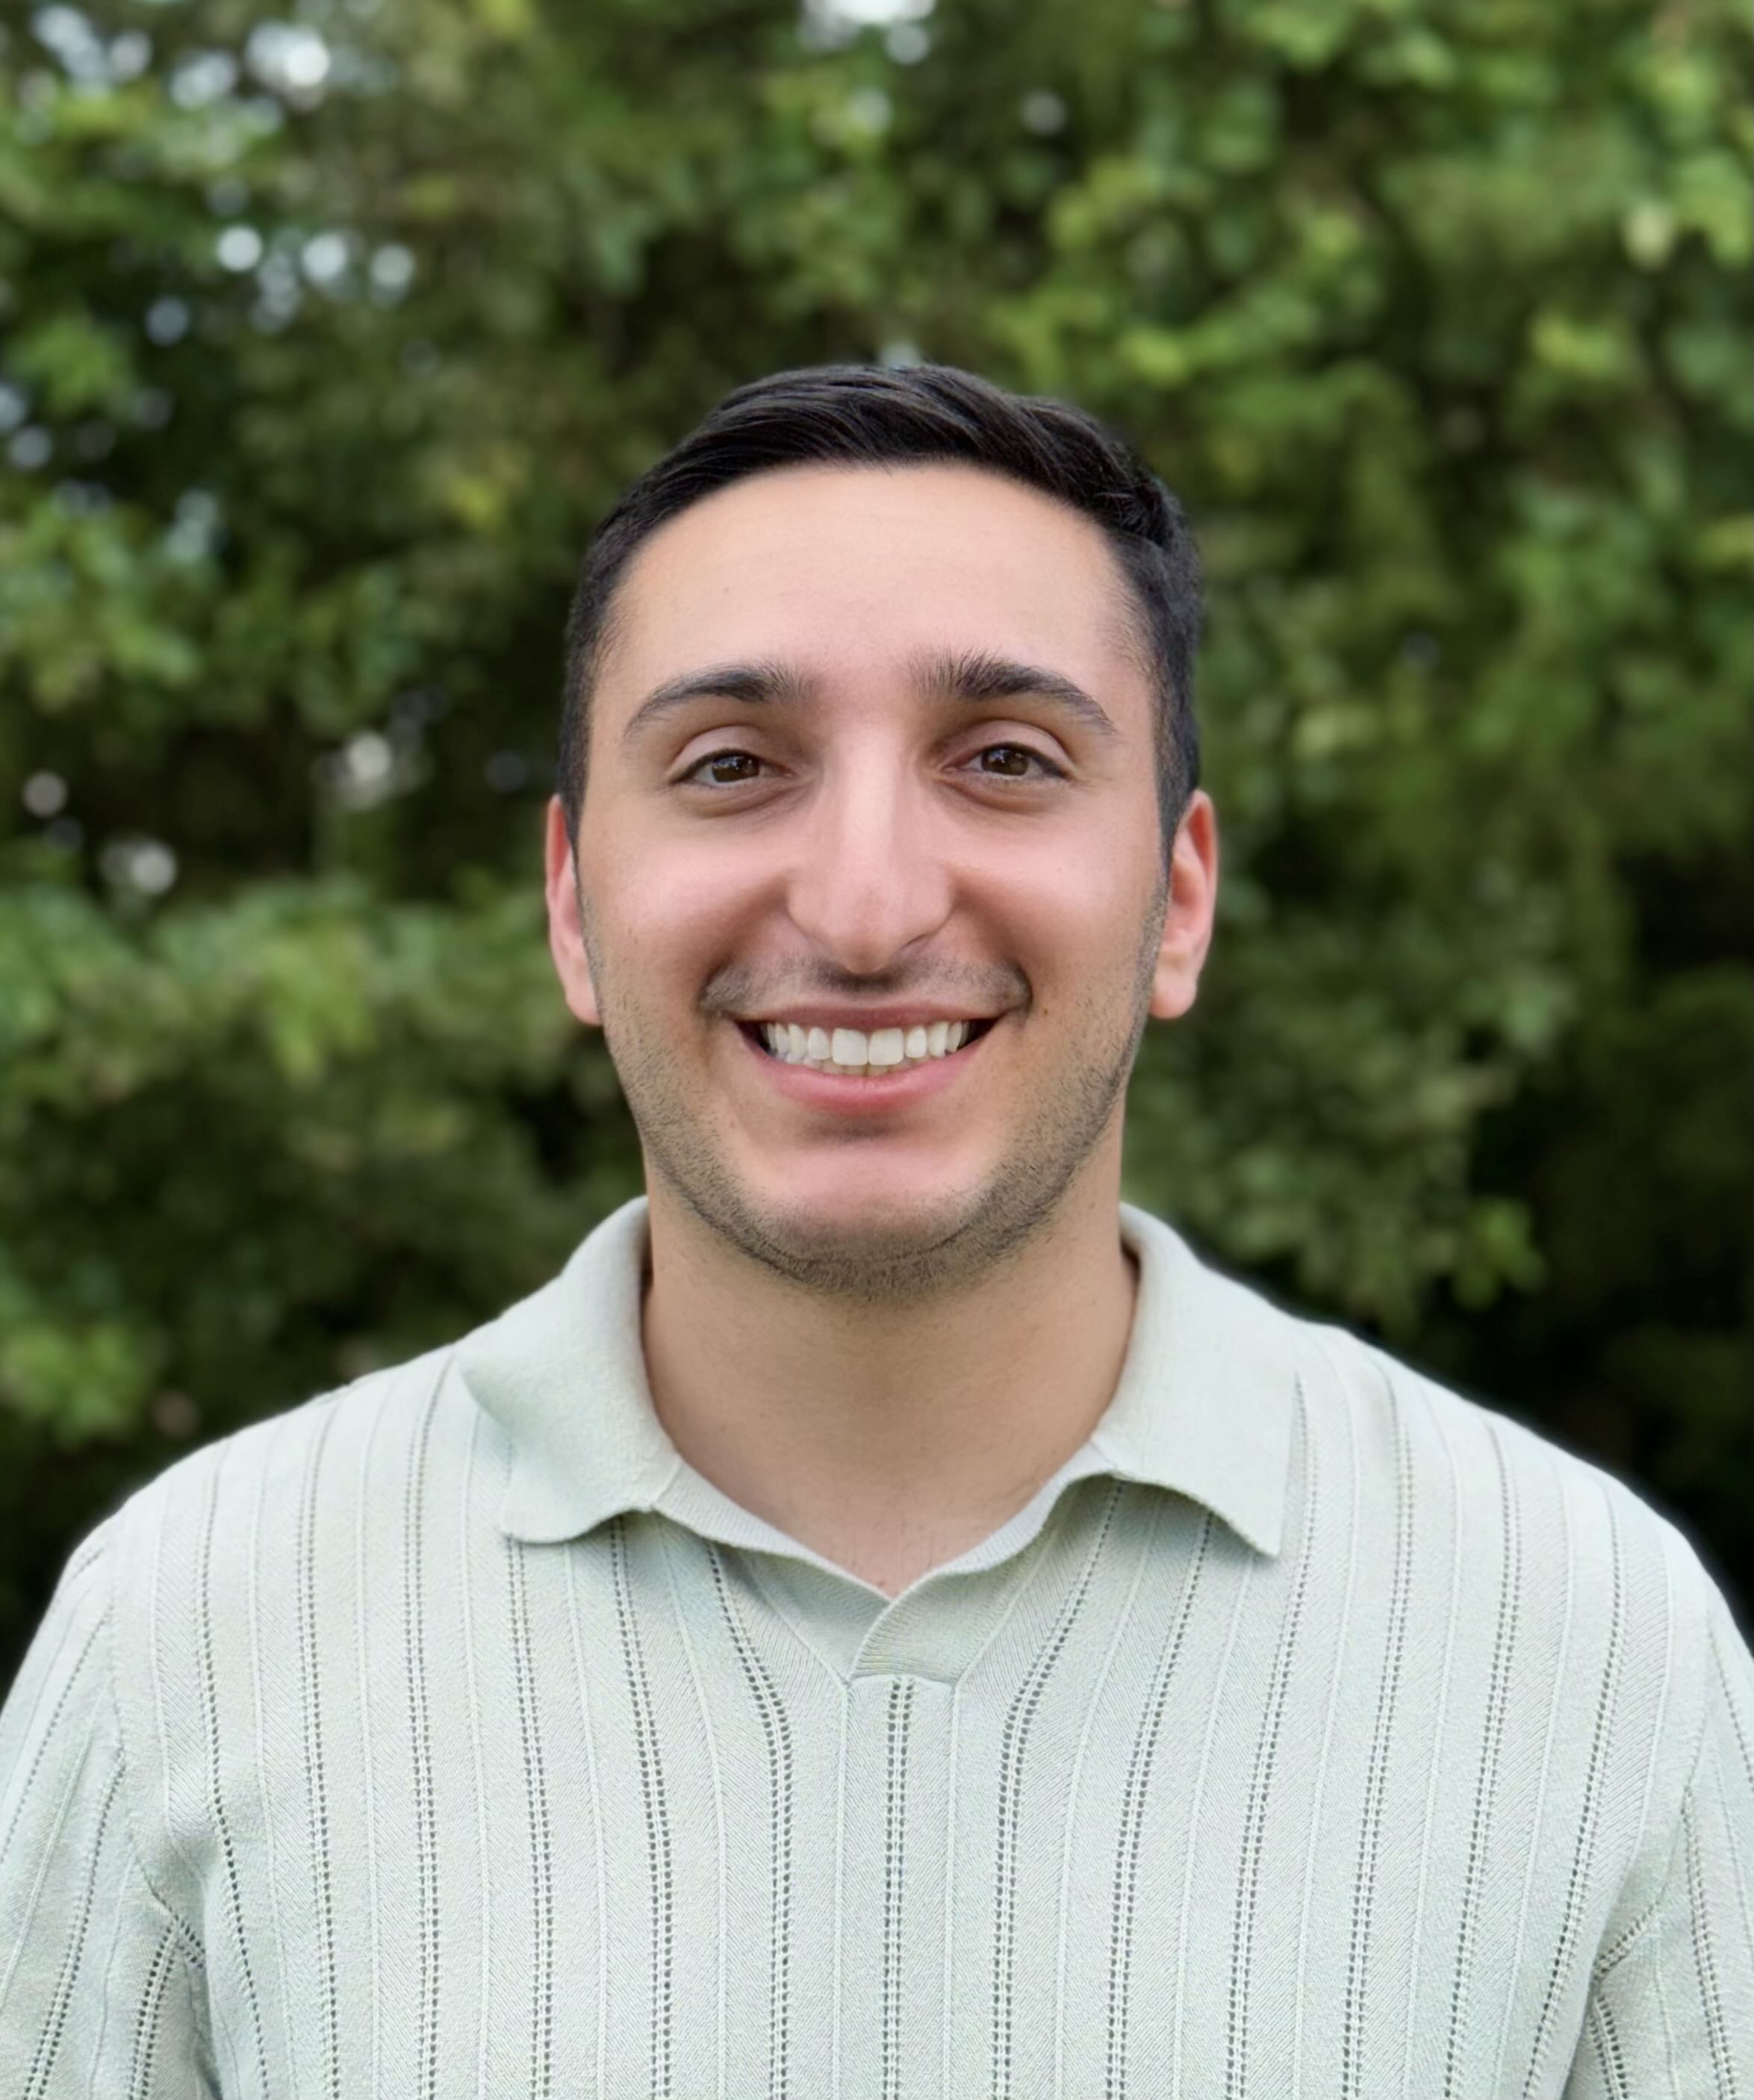
\includegraphics[width=0.5\linewidth]{figures/headshot.png}
    % Includes an image from your figures folder
    % width controls size (0.5 = half the page width)

    \caption[Short caption. This short caption appears in the LIST OF FIGURES]{\textbf{Short caption. This short caption appears in the LIST OF FIGURES} This is the full caption that appears under the figure. Captions should be descriptive enough to understand the figure without referring back to the main text.}
    % Optional [] = short caption for list of figures
    % {} = full caption shown in document

    \label{fig:example_figure}
    % Label MUST come after caption for proper referencing
\end{figure}

\section{Example Section}

Lorem ipsum dolor sit amet, consectetur adipiscing elit.\supercite{example_reference_2}

An example glossary term is \gls{HMSC}.

% \gls{} pulls from your glossary file
% First use = full term, later uses = abbreviated
% In PDFs, this often supports hover/tooltip behavior

Methods chapters often include subsections such as Participants, Data Acquisition, Preprocessing, and Statistical Analysis. These can be created using \texttt{\textbackslash subsection\{\}} to maintain a clear hierarchy.

\subsection{Example Subsection}

Lorem ipsum dolor sit amet, consectetur adipiscing elit.

Example inline math: $p < 0.05$

% Inline math uses $...$ and is embedded within text

Example display math:

\[
y = mx + b
\]

% Display math centers the equation and is used for emphasis or formal definitions

Sed nisi. Nulla quis sem at nibh elementum imperdiet. Duis sagittis ipsum.

\chapter{Manuscript 1}\label{chap:manuscript_1}

% Example manuscript-style chapter demonstrating advanced LaTeX features

\section{Introduction}

Maecenas pulvinar, enim aliquam porttitor tempus, dolor nibh accumsan libero, id scelerisque ligula nibh vitae metus. Vivamus fringilla, tellus nec sodales faucibus, ex neque mollis lorem, vel aliquet elit justo et quam. Cras non ultrices eros. Nulla scelerisque suscipit accumsan. Duis neque mi, suscipit et felis quis, finibus tincidunt ex. Etiam non enim ut nulla vehicula vestibulum. Duis ultrices odio a commodo interdum. Fusce lacinia sodales laoreet.

Nulla sit amet vulputate diam. Etiam quis finibus turpis. Vestibulum ac auctor elit, nec faucibus massa. Morbi ullamcorper felis nisi, et elementum nibh porta a. Duis vestibulum orci ex, eget porttitor felis malesuada sed. Phasellus eros arcu, elementum at consequat sed, placerat et velit. Vivamus nisi tellus, placerat sed velit id, pellentesque mattis ex.

\section{Methods}

\subsection*{Participants}

Participants were greater than or equal to, which can also be written as $\geq 18$.

\subsection*{Behavioral Measures}

Integer purus est, hendrerit eget mollis at, maximus in elit. Phasellus eu lacinia eros. In ac ultricies nunc. Aenean malesuada commodo lacus id consectetur. Fusce facilisis hendrerit sem. Nunc sed faucibus tortor. Nullam tincidunt, felis sed mollis hendrerit, massa elit egestas lorem, quis dapibus leo diam quis nibh. Donec neque orci, molestie non velit ut, pulvinar elementum leo. Sed neque quam, ultricies vitae tortor a, tincidunt lacinia libero. Morbi vitae condimentum mauris. Vivamus venenatis erat ullamcorper, fermentum est vel, laoreet magna. Aliquam elementum lorem

\subsection*{Example Figure}

As shown in \textbf{\autoref{fig:example_main}}, figures are included using the standard \texttt{figure} environment.

\begin{figure}[htbp]
\centering
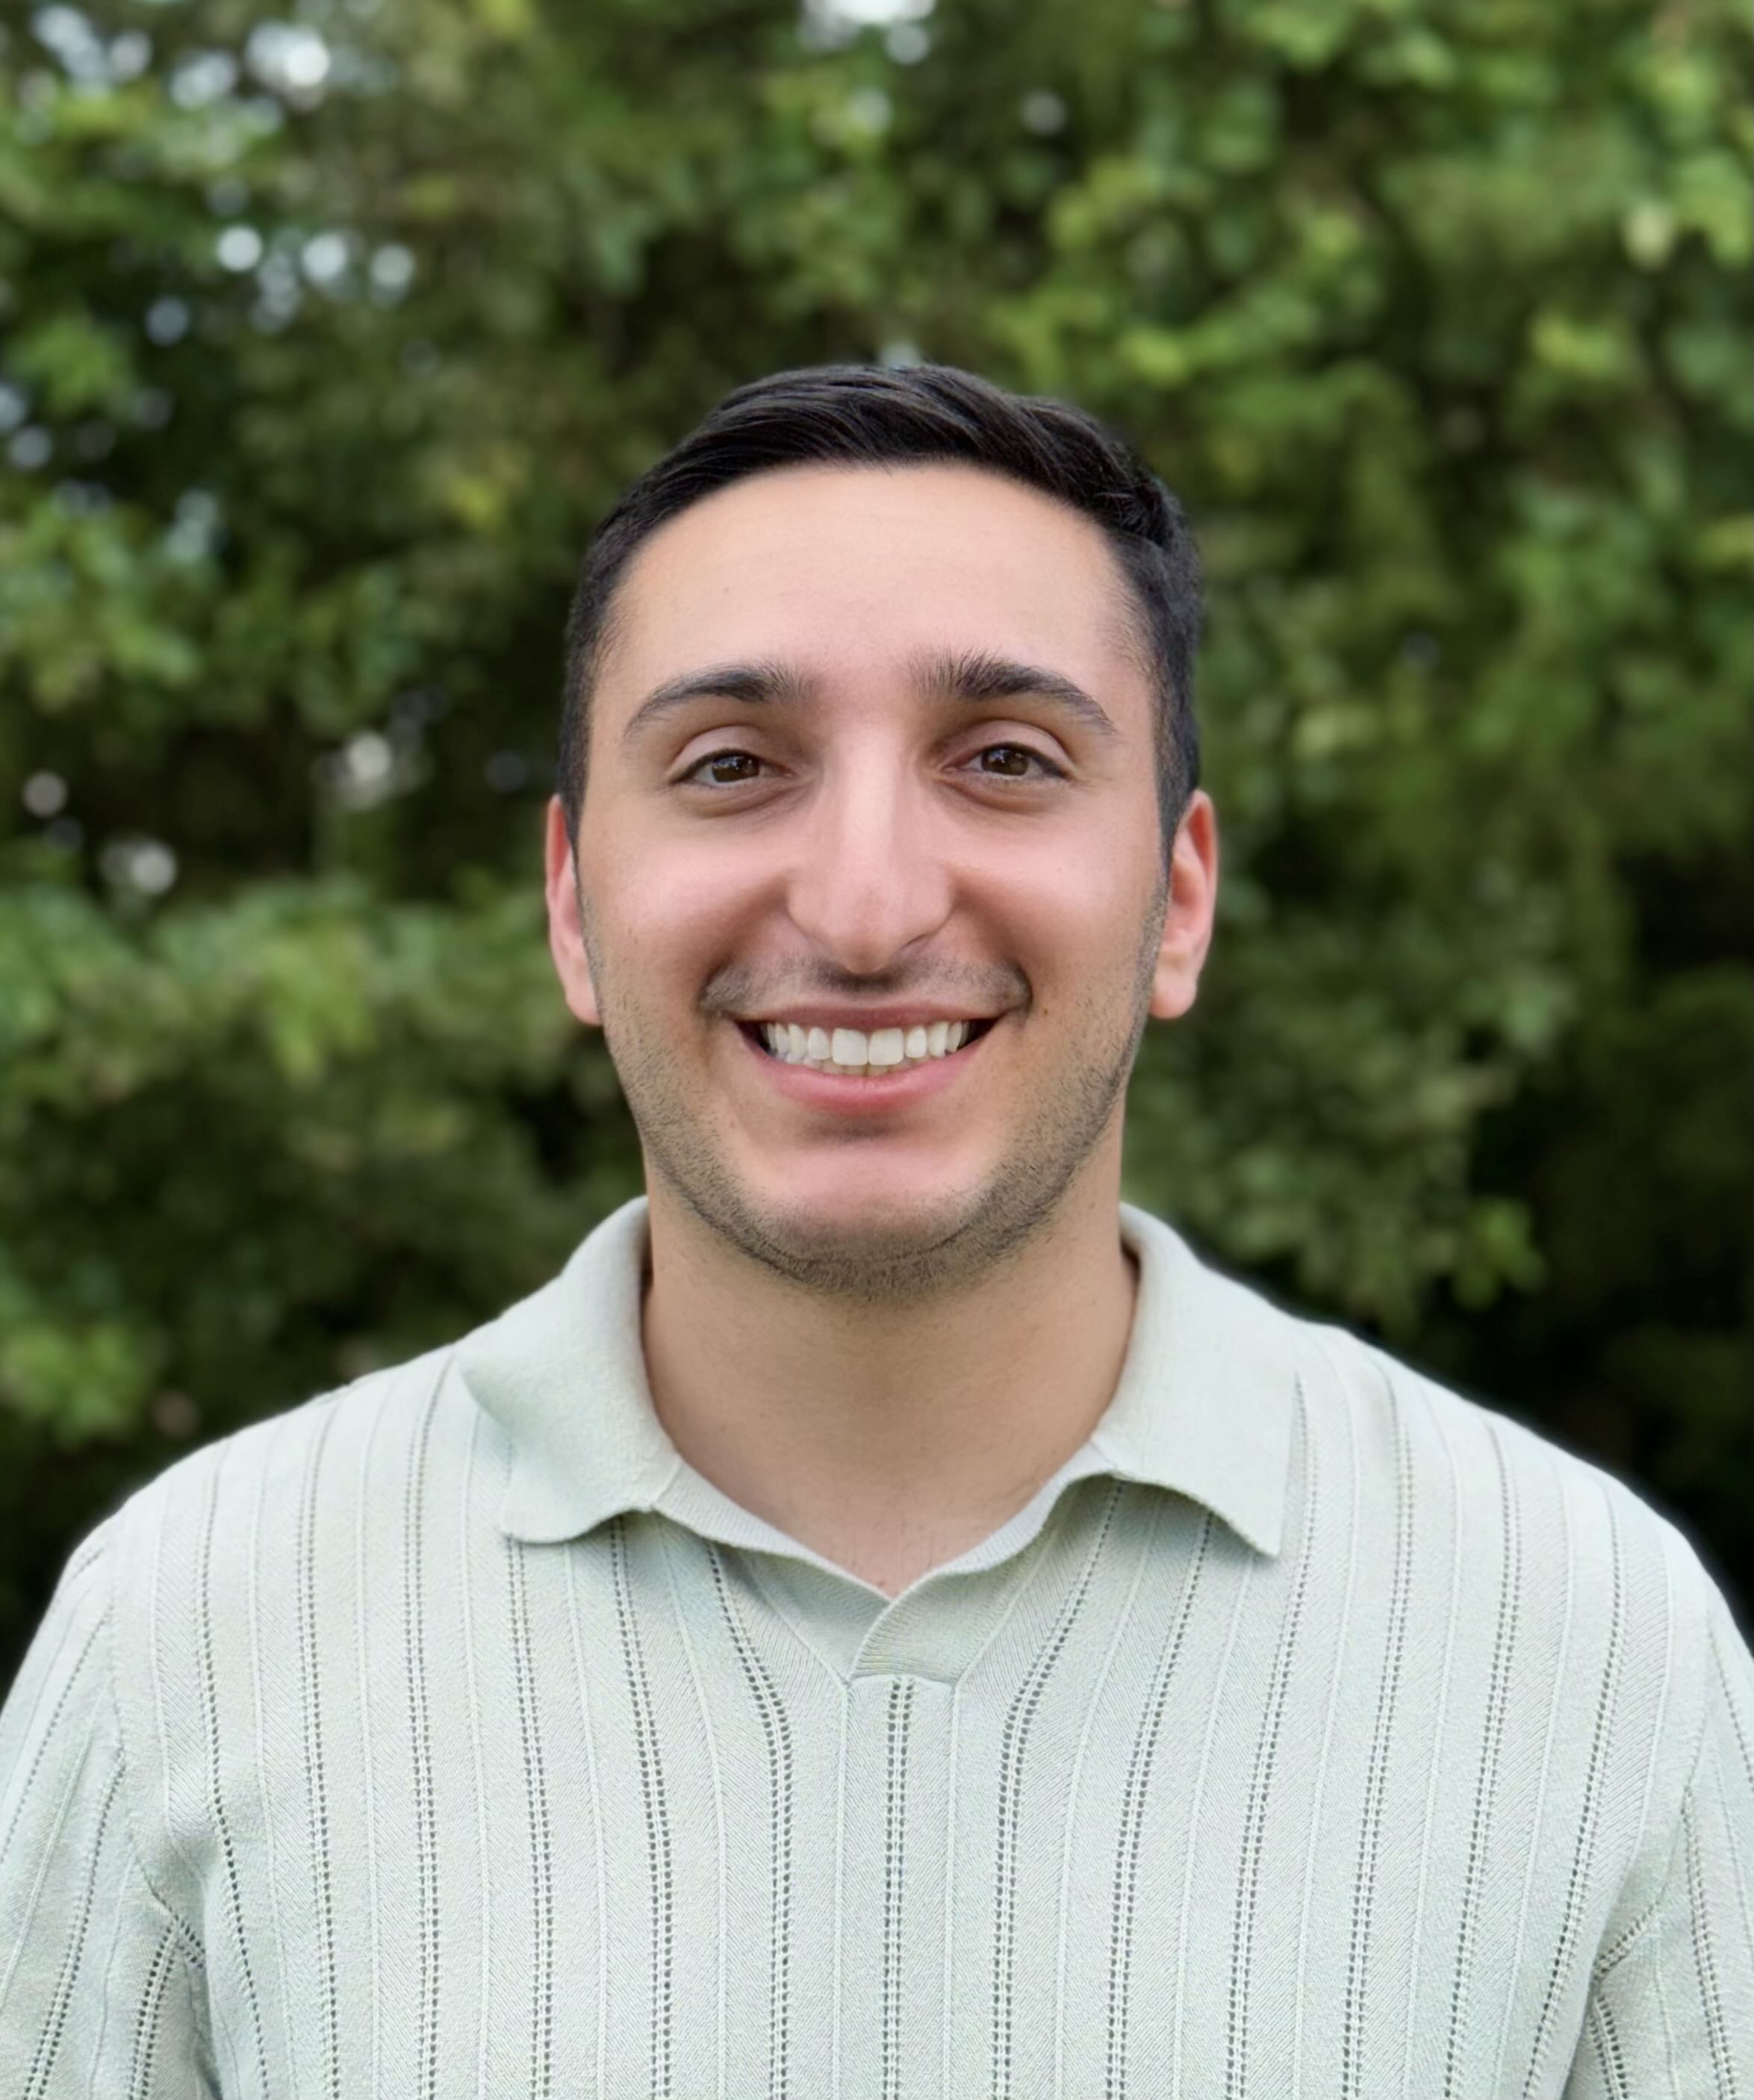
\includegraphics[width=0.3\linewidth]{figures/headshot.png}
\caption[Example figure. Again here is the short caption]{\textbf{Example figure. Again here is the short caption} This demonstrates how to include and reference a figure in a manuscript chapter.}
\label{fig:example_main}
\end{figure}

\subsection*{Example Math}

Inline statistical reporting: $p < 0.05$

Display math:

\[
F_{(1,22)} = 7.12, \quad p < 0.05
\]

\section{Results}

Nulla ut elit lorem. Aenean lorem metus, venenatis sed vehicula eu, rhoncus eu dui. Nam cursus bibendum hendrerit. Phasellus elementum consequat felis ac ornare. Ut eget neque in orci cursus ullamcorper eget vitae urna. Mauris risus mi, tincidunt vitae neque id, auctor dignissim turpis. Integer iaculis blandit lectus pulvinar ullamcorper. Morbi at nulla ac mauris tristique tincidunt eu vitae ante.

 (\textbf{\autoref{fig:example_main}}).

Suspendisse vel tincidunt nunc. Aenean feugiat consectetur augue et sagittis. Vivamus elementum, magna a mollis fringilla, lorem elit posuere (see \textbf{\suppautoref{supfig:example_supp}}).

\section{Discussion}

Suspendisse congue elementum est, non lobortis massa rhoncus a. Nulla facilisi. In in faucibus nisi. Proin metus magna, tristique quis consequat vestibulum, sollicitudin quis diam. Nulla in dapibus mi, vel vulputate diam. In tellus dui, mattis facilisis nulla sed, pulvinar gravida mi. Nullam placerat felis eget diam tincidunt, in vestibulum lectus venenatis. Etiam a viverra massa. Quisque sagittis pulvinar iaculis. Aliquam erat volutpat. Aliquam non condimentum tellus. Nunc vel tortor at tellus cursus ultricies. Donec ut convallis metus.

Vestibulum egestas pellentesque tortor vitae interdum. Vivamus sed nulla ornare, ultricies odio id, aliquam massa. Sed auctor mollis lacus eu cursus. Praesent congue nibh libero, porta finibus lacus eleifend et. In in lectus nec odio sodales accumsan in eget tortor. Suspendisse cursus ligula et diam bibendum, et bibendum enim lacinia. Quisque lobortis augue non congue tincidunt. Duis ut neque a magna fringilla tempus ut non felis. Vivamus auctor leo nec nulla porta malesuada. Maecenas id interdum tortor.

\section{Conclusion}

Nam efficitur euismod tincidunt. Sed lacinia urna id libero dapibus, non vehicula urna eleifend. Fusce elementum finibus rhoncus. Vestibulum nunc mi, scelerisque in volutpat gravida, aliquam a est. Duis ante dui, vehicula ut cursus maximus, sollicitudin ut purus. Vestibulum convallis felis nisl, in suscipit elit tincidunt vitae. Cras orci mi, rutrum non varius vel, rutrum ultrices sem. Aenean lobortis, sapien ut mal

% ======================
% SUPPLEMENTARY FIGURES
% ======================

\newpage
\section*{Supplementary Figures}

Supplementary figures provide additional analyses supporting the main results.

\begin{supfigure}[H]
\centering
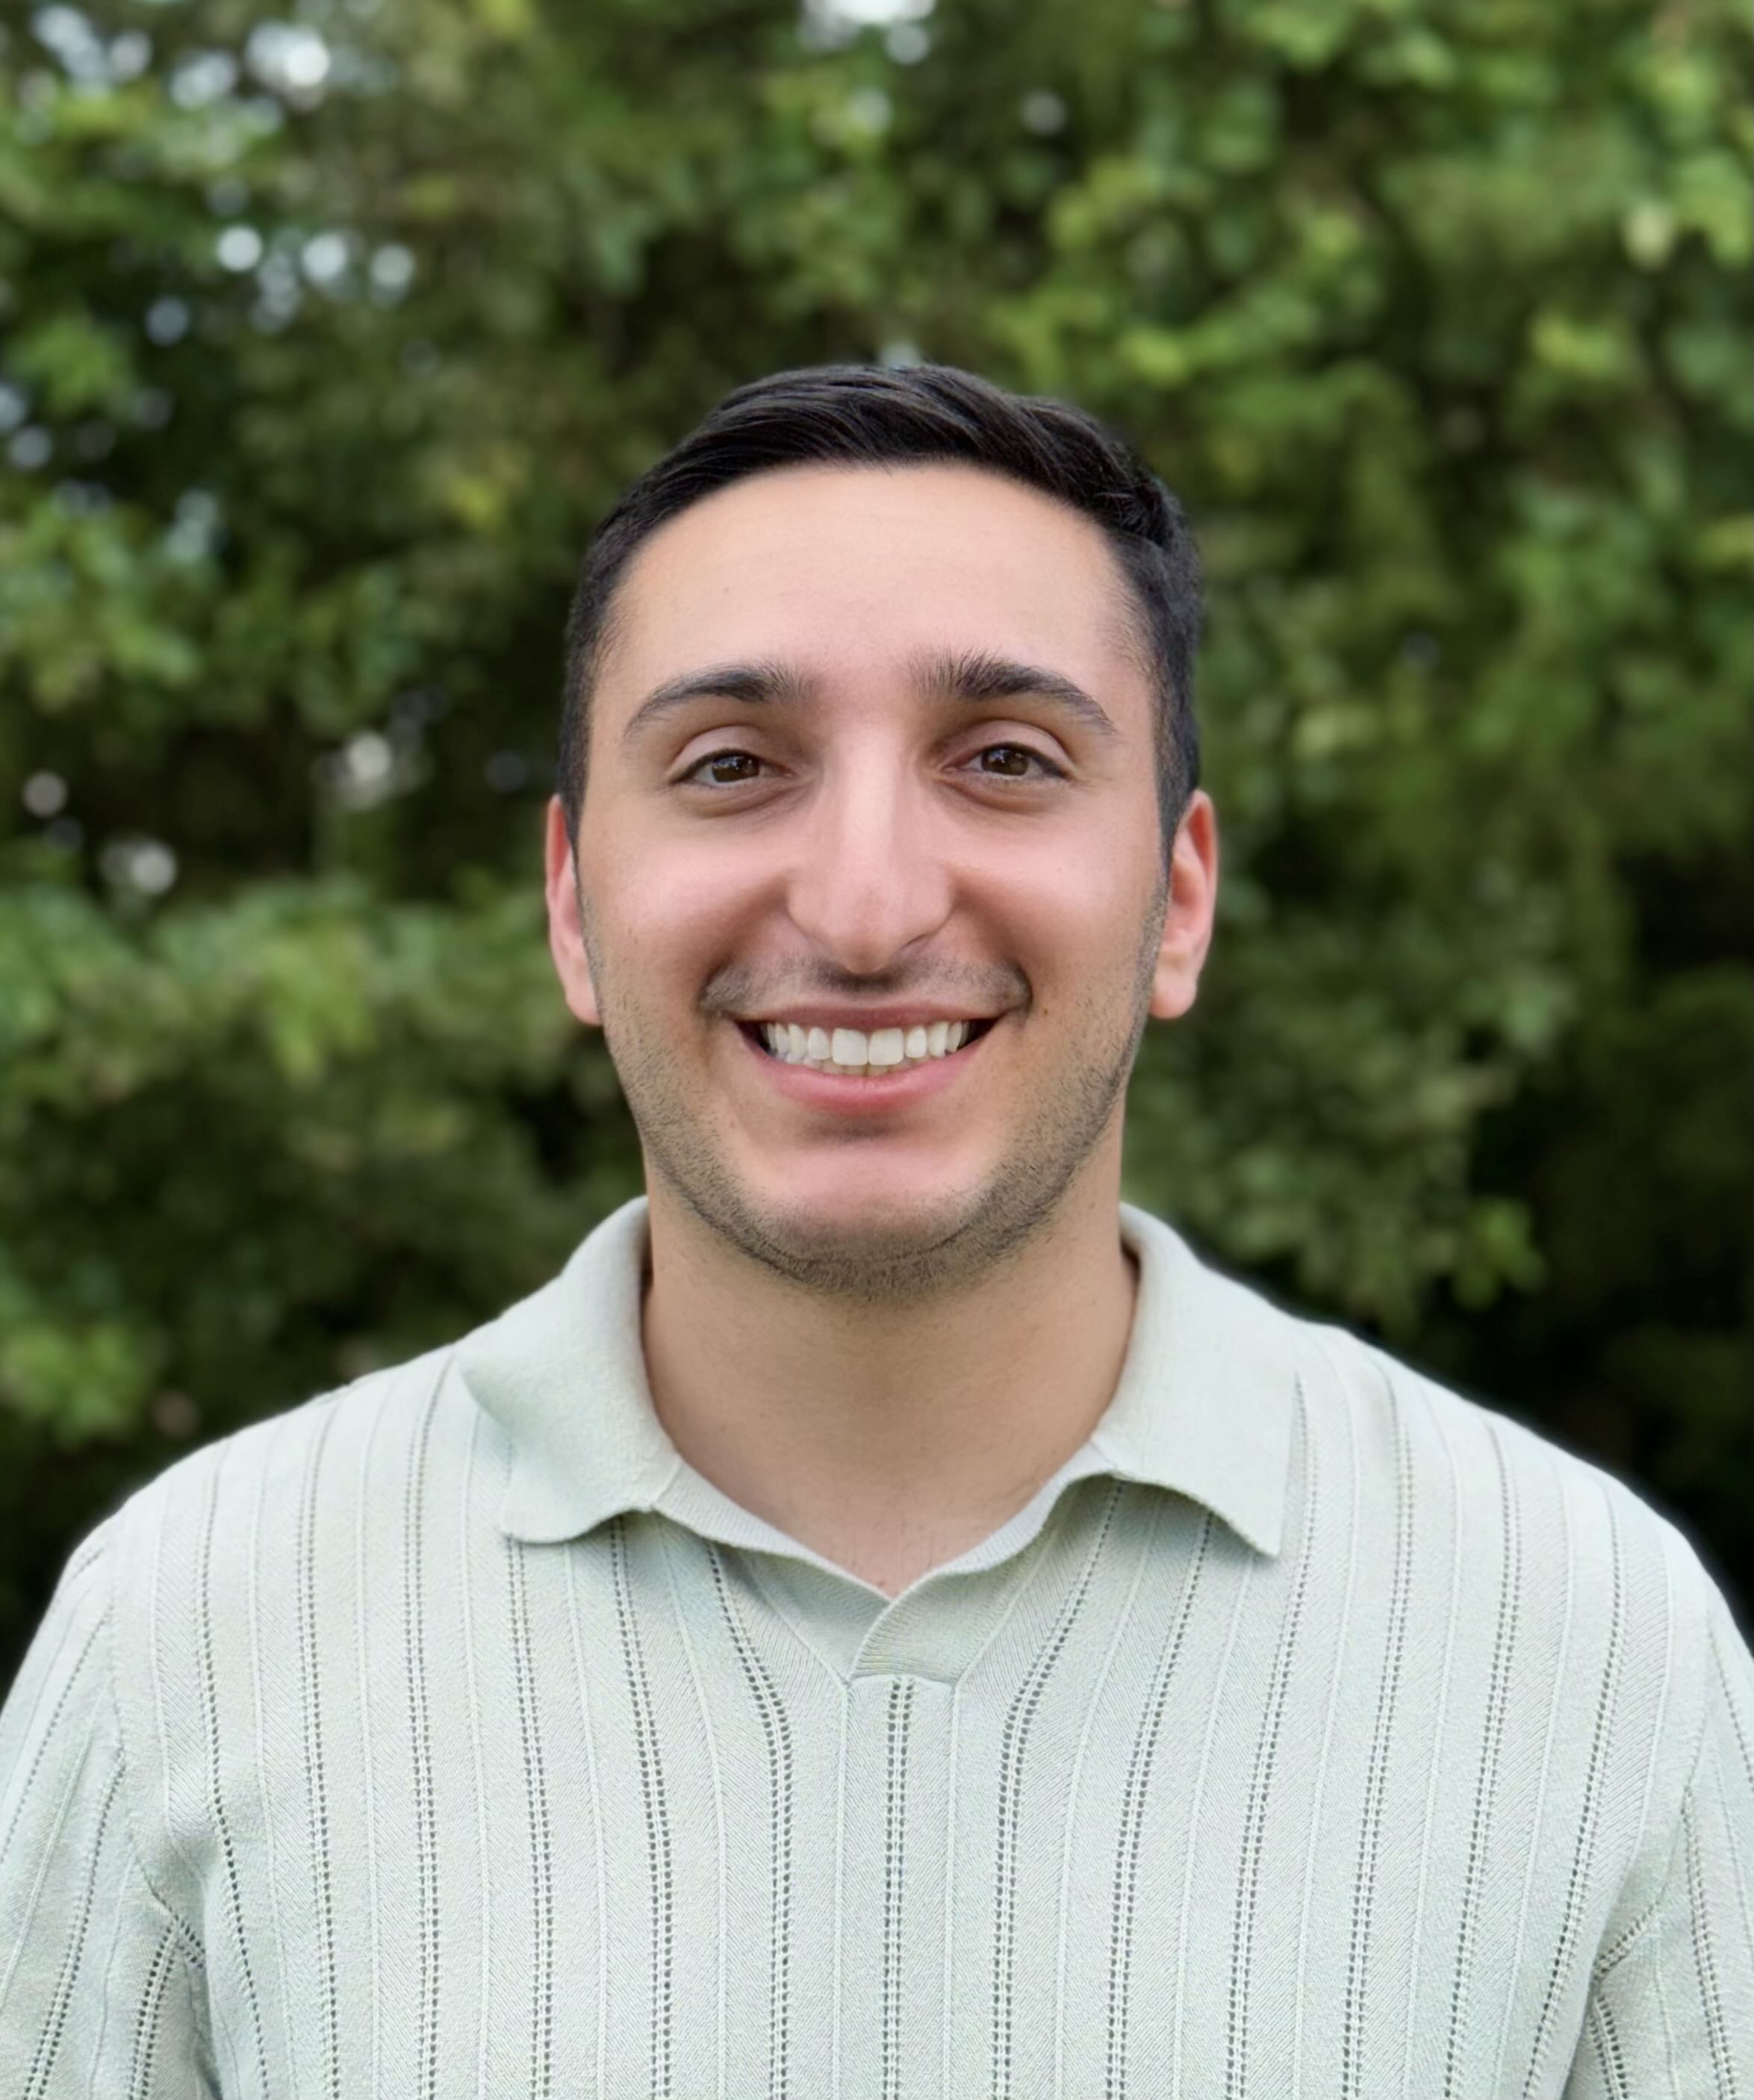
\includegraphics[width=\linewidth]{figures/headshot.png}
\caption[Example supplementary figure]{\textbf{Example supplementary figure.} This demonstrates how to include and reference supplementary material using a custom \texttt{supfigure} environment.}
\label{supfig:example_supp}
\end{supfigure}
\chapter{Manuscript 2}\label{chap:manuscript_2}

% Example manuscript-style chapter demonstrating advanced LaTeX features

\section{Introduction}

Maecenas pulvinar, enim aliquam porttitor tempus, dolor nibh accumsan libero, id scelerisque ligula nibh vitae metus. Vivamus fringilla, tellus nec sodales faucibus, ex neque mollis lorem, vel aliquet elit justo et quam. Cras non ultrices eros. Nulla scelerisque suscipit accumsan. Duis neque mi, suscipit et felis quis, finibus tincidunt ex. Etiam non enim ut nulla vehicula vestibulum. Duis ultrices odio a commodo interdum. Fusce lacinia sodales laoreet.

\section{Methods}

\subsection*{Participants}

Participants were greater than or equal to, which can also be written as $\geq 18$.

\subsection*{Behavioral Measures}

Integer purus est, hendrerit eget mollis at, maximus in elit. Phasellus eu lacinia eros. In ac ultricies nunc. Aenean malesuada commodo lacus id consectetur. Fusce facilisis hendrerit sem. Nunc sed faucibus tortor. Nullam tincidunt, felis sed mollis hendrerit, massa elit egestas lorem, quis dapibus leo diam quis nibh. Donec neque orci, molestie non velit ut, pulvinar elementum leo. Sed neque quam, ultricies vitae tortor a, tincidunt lacinia libero. Morbi vitae condimentum mauris. Vivamus venenatis erat ullamcorper, fermentum est vel, laoreet magna. Aliquam elementum lorem

\section{Results}

Nulla ut elit lorem. Aenean lorem metus, venenatis sed vehicula eu, rhoncus eu dui. Nam cursus bibendum hendrerit. Phasellus elementum consequat felis ac ornare. Ut eget neque in orci cursus ullamcorper eget vitae urna. Mauris risus mi, tincidunt vitae neque id, auctor dignissim turpis. Integer iaculis blandit lectus pulvinar ullamcorper. Morbi at nulla ac mauris tristique tincidunt eu vitae ante. .



\section{Discussion}

Suspendisse congue elementum est, non lobortis massa rhoncus a. Nulla facilisi. In in faucibus nisi. Proin metus magna, tristique quis consequat vestibulum, sollicitudin quis diam. Nulla in dapibus mi, vel vulputate diam. In tellus dui, mattis facilisis nulla sed, pulvinar gravida mi. Nullam placerat felis eget diam tincidunt, in vestibulum lectus venenatis. Etiam a viverra massa. Quisque sagittis pulvinar iaculis. Aliquam erat volutpat. Aliquam non condimentum tellus. Nunc vel tortor at tellus cursus ultricies. Donec ut convallis metus.


\section{Conclusion}

Nam efficitur euismod tincidunt. Sed lacinia urna id libero dapibus, non vehicula urna eleifend. Fusce elementum finibus rhoncus. Vestibulum nunc mi, scelerisque in volutpat gravida, aliquam a est. Duis ante dui, vehicula ut cursus maximus, sollicitudin ut purus. Vestibulum convallis felis nisl, in suscipit elit tincidunt vitae. Cras orci mi, rutrum non varius vel, rutrum ultrices sem. Aenean lobortis, sapien ut mal

\input{ch6}
\chapter{Synthesis}\label{chap:synthesis}

\section{Introduction}
Etiam dictum id nisl sit amet scelerisque. Duis imperdiet mollis ante eu gravida. Donec iaculis consequat libero, at dictum neque. Proin lectus neque, consequat sit amet posuere eget, molestie id ex. Suspendisse pharetra imperdiet est in tristique. Morbi blandit lobortis lacus, quis faucibus turpis facilisis vel. Suspendisse ac rutrum ante. Nullam risus dui, tempor sit amet rhoncus ut, euismod eget purus. Donec felis dui, ultricies sed ipsum tincidunt, viverra elementum odio. Orci varius natoque penatibus et magnis dis parturient montes, nascetur ridiculus mus. Nunc varius est non nisl egestas, a tristique lorem porta.

Pellentesque condimentum aliquet malesuada. Donec eu nisl in magna mattis ultrices. Vivamus ut congue augue. Maecenas eu condimentum mi. Etiam a varius felis, pretium maximus elit. Suspendisse quis augue feugiat, convallis orci vel, commodo est. Curabitur vitae metus bibendum, finibus orci quis, vulputate est. Cras sed sem eget lacus pellentesque ultrices. Vivamus et porta leo. Quisque bibendum risus lacus, at rhoncus libero pharetra interdum. Sed vitae finibus ipsum. Vivamus eu viverra nunc, nec fringilla tellus. Vestibulum ante ipsum primis in faucibus orci luctus et ultrices posuere cubilia curae;

Duis commodo dignissim turpis, vitae gravida diam tempor vel. Nunc tellus nisl, egestas vitae magna vitae, iaculis venenatis risus. Donec vel nisi efficitur, fringilla purus in, fringilla dolor. Nulla a nunc congue, dictum leo ac, facilisis nisi. Sed vitae diam arcu. Nam elementum laoreet nibh volutpat iaculis. Etiam in nulla arcu. Curabitur non eros ut nulla interdum tristique vel et dolor. Donec id bibendum metus, ac suscipit ligula. Vestibulum varius accumsan elit, eu vestibulum lorem scelerisque sit amet. Donec aliquet orci at felis fringilla consectetur. Sed sit amet pulvinar est, a mattis magna. Donec ornare sapien at nulla bibendum bibendum. Proin a interdum massa. Ut sit amet dolor sollicitudin, viverra risus at, imperdiet lorem.

\section{Main Findings of Specific Aim 1}

Phasellus auctor, ipsum nec dictum vehicula, felis magna tristique mi, ac rutrum est justo id ipsum. Suspendisse dolor arcu, dignissim id sapien in, euismod lobortis odio. Curabitur quis turpis elementum, molestie purus et, tincidunt magna. Donec vitae pulvinar diam. Etiam vulputate consequat enim vel auctor. Fusce convallis scelerisque lorem non fringilla. Quisque tempus augue id erat lacinia, et consectetur magna porta.

Suspendisse tincidunt, ligula sed volutpat accumsan, lectus ipsum eleifend quam, sit amet malesuada tellus neque non eros. Quisque sed tellus diam. Sed ut odio finibus diam mollis ultrices. Praesent at sodales quam. Donec ultricies sapien posuere accumsan sodales. Nunc luctus est dolor, ultricies facilisis nibh tempus et. 

\section{Main Findings of Specific Aim 2}

Mauris tincidunt sodales risus, ut varius massa viverra at. Sed consequat nunc ex, at laoreet nibh porttitor eget. Vestibulum vel molestie lectus, eu cursus ligula. Donec id egestas justo. Class aptent taciti sociosqu ad litora torquent per conubia nostra, per inceptos himenaeos. Suspendisse quis facilisis lacus. Nam eget elit eget quam tempus posuere. Aenean finibus, odio vel congue facilisis, justo elit scelerisque ipsum, sit amet consequat purus quam et ligula.

Etiam varius hendrerit magna vel condimentum. Nulla justo odio, fringilla id eros nec, ultrices sagittis eros. Morbi imperdiet dictum eros, auctor porta metus facilisis vitae. Maecenas purus nunc, pharetra vehicula urna sit amet, efficitur lacinia neque. Vestibulum fringilla, lectus et tempus sagittis, lacus justo blandit ipsum, ut consectetur justo mi eget velit. Cras elementum purus vel nulla fermentum, a faucibus turpis varius. Vestibulum consequat quam turpis, id congue tellus varius eu. Curabitur egestas mattis sagittis. Nulla quis faucibus arcu, cursus sagittis elit. Duis congue venenatis hendrerit. Ut in erat vitae nunc lacinia congue at non risus. Sed id leo volutpat, dignissim mi et, auctor nibh.


\section{Main Findings of Specific Aim 3}
Vestibulum interdum vulputate lorem ultrices elementum. Duis et est iaculis, porttitor dolor vitae, vehicula velit. Ut ultricies odio quis nisl feugiat, eu semper ipsum semper. Donec tempor augue dui, quis commodo eros lobortis quis. Integer aliquam, lorem a mollis dignissim, metus ante hendrerit augue, et suscipit risus lectus non diam. Pellentesque eleifend a augue eget scelerisque. Nullam eleifend maximus commodo. Suspendisse luctus aliquet quam at iaculis. Integer quis auctor ante, vel dapibus turpis. Nunc imperdiet leo pharetra cursus ultricies. Nulla tincidunt sapien et leo rhoncus, non placerat risus elementum. Ut id interdum magna. Duis a lectus eu lacus fringilla finibus.

Ut euismod sapien sed semper posuere. Praesent in sodales urna, at commodo magna. Nulla iaculis mattis enim, id dapibus mauris hendrerit eu. Fusce aliquet, felis quis vehicula eleifend, enim quam pellentesque metus, ultrices fringilla sapien risus vel nunc. Nunc sit amet risus elit. Integer a mi libero. Pellentesque id libero nec leo finibus ornare. In nibh lectus, efficitur nec aliquam in, euismod in mi. Cras tincidunt justo arcu, eget malesuada elit tincidunt ac. Phasellus eleifend erat nec metus pretium, non ultricies augue maximus.

\section{Integrative Framework}

Sed malesuada malesuada justo, lacinia viverra lacus gravida et. Morbi hendrerit blandit orci ac feugiat. Etiam auctor pellentesque eros id facilisis. Etiam egestas sagittis mauris nec dictum. Donec pellentesque odio vitae odio pharetra vehicula. Vivamus quis sapien auctor, posuere dolor in, bibendum lorem. Aliquam erat volutpat. Aenean malesuada mauris id justo aliquam vehicula. Nulla elementum ornare nulla non dapibus. Quisque suscipit in urna nec dictum. Pellentesque eu est massa.

Suspendisse eu ultrices dolor, vel facilisis lectus. Pellentesque ut semper ante, vel faucibus massa. Quisque tincidunt blandit augue et eleifend. Morbi congue dui ornare erat euismod, at fringilla nibh consectetur. Cras sodales euismod risus dapibus porttitor. Vestibulum lectus risus, pellentesque eget fermentum at, suscipit at arcu. Duis hendrerit efficitur scelerisque. Aenean consectetur lacinia nulla. Donec vel dui felis. Sed sollicitudin ac magna eu dignissim. Nullam et elit eget dolor commodo sodales bibendum eget turpis. In porttitor turpis sed luctus placerat. Donec mollis quam purus, vel ornare dolor hendrerit vel. Suspendisse sit amet magna nec augue convallis tincidunt. Sed fringilla luctus urna vel mollis. Aliquam ac volutpat quam, vel laoreet ipsum.


\section{Clinical Implications and Future Directions}

Sed ornare urna sit amet suscipit vehicula. Nunc sit amet lobortis diam. Nam rhoncus nisi sed auctor commodo. Nunc bibendum quam quis lacus rhoncus pellentesque. Cras interdum urna eu nisi aliquet, quis luctus eros lobortis. Nullam vehicula fermentum sem, et auctor odio facilisis id. Fusce sem nibh, aliquam quis urna nec, semper vulputate justo.

Nullam sed urna interdum, bibendum nisl a, vulputate ex. Vestibulum dapibus malesuada libero, vitae malesuada velit ornare in. Sed aliquam lorem non efficitur pharetra. Vestibulum tempor leo at dolor hendrerit, sed semper justo placerat. Fusce dapibus tempor quam sed hendrerit. Aliquam auctor velit id tellus aliquam, vitae maximus ex convallis. Aliquam viverra, eros nec varius ultrices, lorem massa consequat turpis, nec sodales justo est a nulla. In mattis pretium nulla, eu congue sem molestie vitae. Suspendisse quis suscipit nisi. Fusce hendrerit vitae risus eget imperdiet.

\section{Concluding Remarks}

Aliquam sit amet mollis eros. Vivamus lobortis odio ac nunc dignissim fermentum ultrices id turpis. Vivamus rutrum dolor a risus porta, non mattis leo tempor. Donec sodales nisl justo, eu dignissim elit ornare malesuada. Quisque sit amet ante sed tortor convallis pellentesque. Aliquam congue viverra mattis. Nunc lobortis, ex bibendum aliquet hendrerit, tellus justo pretium nisi, vitae cursus metus justo in urna.

Phasellus finibus hendrerit pellentesque. Nullam a lectus nulla. Phasellus tincidunt risus et orci pretium, vel convallis risus rutrum. Fusce varius magna id diam blandit aliquam. Morbi ultricies, nisi fringilla rhoncus faucibus, magna elit blandit diam, non aliquam enim felis et lacus. Nullam id nibh at ligula ornare venenatis a vitae enim. Nunc convallis eleifend interdum. Aliquam a pulvinar libero. Duis cursus dui ligula, at pellentesque metus auctor nec. Donec feugiat, felis vitae posuere laoreet, eros turpis vestibulum nunc, eu tempus nibh libero nec ligula. Mauris iaculis sollicitudin egestas. Morbi egestas nibh vulputate tellus sagittis condimentum nec id turpis. Nam magna nulla, tincidunt a felis quis, sodales finibus mauris. Cras accumsan gravida faucibus. Cras sed tellus nibh. Proin lacinia tellus risus, in mollis nunc accumsan at.

%%%%%%%%%%%%%%%%%%%%%%%%%%%%%%%%%%%%%%%%%%%%%%%%%%
%% APPENDICES
%%%%%%%%%%%%%%%%%%%%%%%%%%%%%%%%%%%%%%%%%%%%%%%%%%

\appendix

% Adjust spacing for appendix titles
\titlespacing{\chapter}{0in}{-.38in}{11pt}

\refstepcounter{chapter}
\chapter*{APPENDIX \thechapter: NAME OF THE APPENDIX}
\addcontentsline{toc}{chapter}{APPENDIX \thechapter: NAME OF THE APPENDIX}

% The appendix is unnumbered (chapter*) but still appears in the Table of Contents
% \refstepcounter ensures correct labeling (APPENDIX A, B, etc.)
\vspace{-22pt}

\section*{Purpose of the Appendix}

This appendix provides additional clarification, supporting analyses, or extended methodological details that complement the main text but are not essential to the primary narrative.


\refstepcounter{chapter}
\chapter*{APPENDIX \thechapter: NAME OF THE OTHER APPENDIX}
\addcontentsline{toc}{chapter}{APPENDIX \thechapter: NAME OF THE OTHER APPENDIX}

% The appendix is unnumbered (chapter*) but still appears in the Table of Contents
% \refstepcounter ensures correct labeling (APPENDIX A, B, etc.)
\vspace{-22pt}

\section*{This is where the other appendix would go}

Integer id neque ultricies, tincidunt dolor eget, faucibus massa. Integer pretium elementum eros et congue. Nulla vitae nunc facilisis, imperdiet neque eu, feugiat sem. Curabitur vehicula laoreet tristique. Nullam mattis vehicula auctor. Morbi et magna leo. Maecenas vel molestie orci, ac malesuada justo. Proin posuere turpis id justo aliquet, nec porta ligula mollis. In ac euismod libero. Sed sapien tortor, pretium at consequat eget, porttitor id leo. Vivamus dapibus lorem lectus, id tristique purus dictum quis. Mauris eu luctus tortor.

Donec ut ex nunc. Quisque eu dui a arcu fermentum maximus. Curabitur mollis felis at laoreet posuere. Sed nulla nunc, pharetra vitae viverra nec, ultricies sed nulla. In non urna sed libero sagittis aliquet. Nam tristique, eros quis tincidunt euismod, turpis ante fringilla odio, eu commodo neque risus rhoncus libero. Mauris ante ex, vestibulum quis metus fermentum, vestibulum consequat ipsum.

Mauris cursus ante quis erat convallis, at vulputate lectus faucibus. Suspendisse rutrum nunc vitae tempor convallis. Fusce sed euismod lorem. Mauris tempus risus ullamcorper tellus posuere, nec elementum orci bibendum. Cras sollicitudin ipsum a mattis rutrum. Suspendisse imperdiet metus lorem, vitae tincidunt nulla efficitur et. Nulla nibh turpis, porta nec magna vitae, egestas dictum felis.



%%%%%%%%%%%%%%%%%%%%%%%%%%%%%%%%%%%%%%%%%%%%%%%%%%
%% REFERENCES
%%%%%%%%%%%%%%%%%%%%%%%%%%%%%%%%%%%%%%%%%%%%%%%%%%

\setlength{\bibhang}{0pt}
\setlength{\biblabelsep}{0.5em}

% \clearpage
% \phantomsection

% {\def\chapter*#1{} % suppress bibliograph header.
% \begin{singlespace}
% \addcontentsline{toc}{chapter}{BIBLIOGRAPHY}
% \begin{center}
% \normalfont \textbf{BIBLIOGRAPHY}
% \vspace{17pt}
% \end{center}

% %\bibliographystyle{ieeetr}
% %\bibliography{diss}

% \printbibliography
% \end{singlespace}
% }



\clearpage
\phantomsection

\begin{singlespace}
\printbibliography[title={BIBLIOGRAPHY}, heading=bibintoc]
\end{singlespace}

\end{document}